\documentclass[a4paper,12pt]{article}

\usepackage{graphicx} % Required for inserting images
\usepackage{amsmath,amssymb,amsfonts}
\usepackage{subcaption}
% -----------------------
% Package Imports
% -----------------------

% Set page margins
\usepackage[a4paper, top=1in, bottom=0.8in, left=1.1in, right=0.8in]{geometry}

% Use Times New Roman font
\usepackage{times}

% Add page numbering
\pagestyle{plain}
\usepackage{multirow}
% Enable graphics inclusion
\usepackage{graphicx}
\usepackage{float}
% Enable code listings
\usepackage{listings}
\usepackage{xcolor} % For customizing code colors
% -----------------------
% Section Font Customization
% -----------------------
\usepackage{titlesec} % To customize section font size
\titleformat{\section}
{\normalfont\fontsize{14}{16}\bfseries}{\thesection}{1em}{}

\titleformat{\subsection}
{\normalfont\fontsize{14}{16}\bfseries}{\thesubsection}{1em}{}


% Define MATLAB style for listings
\lstdefinestyle{vscode-light}{
	language=Matlab,
	basicstyle=\ttfamily\footnotesize,
	keywordstyle=\color{black},
	commentstyle=\color{gray},
	stringstyle=\color{red},
	numberstyle=\tiny\color{black},
	numbersep=5pt,
	frame=single,
	backgroundcolor=\color{white!10},
	breaklines=true,
	captionpos=b,
	tabsize=4,
	showstringspaces=false,
	numbers=left,  % Enable line numbering on the left
	stepnumber=1,  % Line numbers increment by 1
	numberfirstline=true, % Number the first line
}
\setlength{\parindent}{0pt}


\begin{document}
	\section{Experiment No. 9}
	
	\section{Experiment Title }
Nonlinear polynomial curve fitting method using MATLAB.
	\section{Objective}
	
	The objectives of this lab are:
	\begin{itemize}
		\item To practice a nonlinear polynomial best curve fitting.
		\item To create a MATLAB program to find the variables according to the degree of the solving equation.
		
	\end{itemize}
	\section{Theory}
	
	Curve fitting, or regression, is the process of constructing a curve or mathematical function that best fits a series of data points, possibly subject to constraints. It is a fundamental technique used in data analysis and modeling.
	
	Curve fitting can be broadly classified into two categories:
	\begin{enumerate}
		\item Linear curve fitting
		\item Nonlinear curve fitting
	\end{enumerate}
	
	Nonlinear curve fitting can further be classified as:
	\begin{itemize}
		\item Exponential curve fitting
		\item Polynomial curve fitting
	\end{itemize}
	
	In this experiment, we focus on polynomial curve fitting. Let us illustrate this method by fitting a given set of data to a quadratic polynomial. Let the quadratic curve be represented by:
	
	\begin{equation}
		y = a_2x^2 + a_1x + a_0 \tag{9.1}
	\end{equation}
	
	For each data point where \( x = x_i \), the left-hand side of Equation (9.1) becomes:
	
	\begin{equation}
		\bar{y}_i = a_2x_i^2 + a_1x_i + a_0 \tag{9.2}
	\end{equation}
	
	The sum of the squares of the deviations (errors) between the actual and estimated values is given by:
	
	\begin{equation}
		S = \sum (y_i - \bar{y}_i)^2 = \sum (y_i - a_2x_i^2 - a_1x_i - a_0)^2 \tag{9.3}
	\end{equation}
	
	To find the best-fitting curve, we minimize \( S \) with respect to the coefficients \( a_0 \), \( a_1 \), and \( a_2 \). This is done by taking the partial derivatives of \( S \) with respect to each coefficient and setting them equal to zero:
	
	\begin{equation}
		n a_0 + a_1 \sum x_i + a_2 \sum x_i^2 = \sum y_i \tag{9.4}
	\end{equation}
	\begin{equation}
		a_0 \sum x_i + a_1 \sum x_i^2 + a_2 \sum x_i^3 = \sum x_i y_i \tag{9.5}
	\end{equation}
	\begin{equation}
		a_0 \sum x_i^2 + a_1 \sum x_i^3 + a_2 \sum x_i^4 = \sum x_i^2 y_i \tag{9.6}
	\end{equation}
	
	These form a system of three linear equations with three unknowns: \( a_0 \), \( a_1 \), and \( a_2 \). Solving this system gives the coefficients of the best-fit quadratic polynomial.
	
	This basic method can be generalized to fit an \( n^{\text{th}} \) order polynomial. In that case, there will be \( n+1 \) simultaneous equations containing \( n+1 \) unknown constants corresponding to the polynomial coefficients.
	
\section{Algorithm}

\textbf{Input:} Data points \( (x, y) \), order of the polynomial \( n \), and number of data points \( m \)

\textbf{Output:} Coefficients of the best-fitting polynomial and visualization of the fitting curve

\begin{enumerate}
	\item Read the order of the polynomial: \( n \)
	
	Set the number of coefficients: \( c_n \leftarrow n + 1 \)
	
	\item Read the \( x \)-values of the data points: \( x \)
	
	Read the \( y \)-values of the data points: \( y \)
	
	\item Read the number of data points: \( m \)
	
	\item \textbf{Constructing the Right-Hand Side of the Linear System (vector \( b \)):}
	
	\begin{enumerate}
		\item For \( i = 1 \) to \( c_n \):
		\begin{enumerate}
			\item Initialize \( \text{sum} \leftarrow 0 \)
			\item For \( j = 1 \) to \( m \):
			\begin{enumerate}
				\item \( \text{sum} \leftarrow \text{sum} + x[j]^{(i - 1)} \cdot y[j] \)
			\end{enumerate}
			\item End For
			\item \( b[i] \leftarrow \text{sum} \)
		\end{enumerate}
		\item End For
	\end{enumerate}
	
	\item \textbf{Constructing the Left-Hand Side of the Linear System (matrix \( C \)):}
	
	\begin{enumerate}
		\item For \( i = 1 \) to \( c_n \):
		\begin{enumerate}
			\item For \( k = 1 \) to \( c_n \):
			\begin{enumerate}
				\item Initialize \( \text{sum} \leftarrow 0 \)
				\item For \( j = 1 \) to \( m \):
				\begin{itemize}
					\item \( \text{sum} \leftarrow \text{sum} + x[j]^{(i + k - 2)} \)
				\end{itemize}
				\item End For
				\item \( C[i, k] \leftarrow \text{sum} \)
			\end{enumerate}
			\item End For
		\end{enumerate}
		\item End For
	\end{enumerate}
	
	\item Compute the coefficient vector: 
	\[
	a \leftarrow C^{-1} \cdot b^T
	\]
	
	\item \textbf{Determining Polynomial Coefficients:}
	
	\begin{enumerate}
		\item For \( i = 1 \) to \( c_n \):
		\[
		a_n[i] \leftarrow a[c_n - i + 1]
		\]
		\item End For
	\end{enumerate}
	
	\item Display the polynomial coefficients \( a_n \)
	
	\item \textbf{Plotting:}
	
	\begin{enumerate}
		\item Generate \( x_1 \leftarrow \text{linspace}(0, \max(x), 100) \)
		
		\item Compute \( y_1 \leftarrow \text{evaluate polynomial } a_n \text{ at } x_1 \)
		
		\item Plot the data points \( (x, y) \) as red circles
		
		\item Plot the fitting curve \( (x_1, y_1) \)
		
		\item Plot the original data points \( (x, y) \)
		
		\item Generate \( x_m \leftarrow \text{evenly spaced points from } 0 \text{ to } 2\pi \)
		
		\item Compute \( y_m \leftarrow \sin(x_m) \)
		
		\item Plot the sine curve \( (x_m, y_m) \)
	\end{enumerate}
	
	\item \textbf{END}
\end{enumerate}

	\newpage
	\subsection{MATLAB Implementation of Polynomial Curve Fitting}
	
	\subsubsection{MATLAB Code:}
	\begin{lstlisting}[style=vscode-light, caption={MATLAB code for Polynomial Curve Fitting} ]
	
	n = input('Enter the order of the polynomial (n): ');
	%n=10;
	cn = n + 1;
	%x = input('Enter the x values  ');
	%y = input('Enter the y values  ');
	x = [0 0.5 1 1.5 2 2.5 3 3.5 4 4.5 5 5.5 6];   
	y = [0 0.4794 0.8414 0.9974 0.9092 0.5984 0.1411 -0.3504 -0.7568 -0.9775 -0.95892 -0.7055 0.2794];  
	m = length(x);  
	b = zeros(cn, 1);
	
	for i = 1:cn
	sum = 0;
	for j = 1:m
	sum = sum + (x(j)^(i - 1)) * y(j);
	end
	b(i) = sum;
	end
	
	c = zeros(cn, cn);
	for i = 1:cn
	for k = 1:cn
	sum = 0;
	for j = 1:m
	sum = sum + x(j)^((i + k) - 2);
	end
	c(i, k) = sum;
	end
	end
	a = inv(c) * b
	
	an = zeros(1, cn);
	for i = 1:cn
	an(i) = a(cn - i + 1);
	end
	
	disp('Polynomial coefficients (highest degree first):');
	disp(an);
	x1 = linspace(0, max(x), 150);
	y1 = polyval(an, x1);
	plot(x, y, 'ro', 'MarkerFaceColor', 'r'); 
	hold on;
	plot(x1, y1, 'b', 'LineWidth', 2);
	legend('Data points', 'Fitted Polynomial');
	title('Polynomial Curve Fitting');
	xlabel('x');
	ylabel('y');
	grid on;
	
	
	
	
		
		
		
		
		
		
	\end{lstlisting}
	
	\newpage
	
	
	\subsection{Output}
	
	\begin{lstlisting}[style=vscode-light, caption={Command Window} ]
	Enter the order of the polynomial (n): 2
	Enter the order of the polynomial (n): 5
	Enter the order of the polynomial (n): 10
	Enter the order of the polynomial (n): 11
	>> 
	\end{lstlisting}
	\subsubsection{Plot Diagram}
\begin{figure}[H]
	\centering
	\begin{subfigure}[t]{0.49\textwidth}
		\centering
		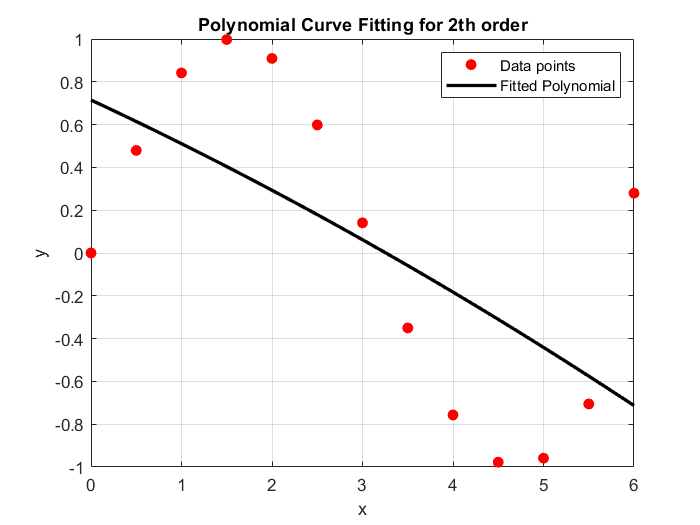
\includegraphics[width=1.1\linewidth]{Images/2}
		\caption{Curve fitting for $2^{nd}$ order}
		\vspace{0.1cm}
	\end{subfigure}
	\hfil
	\begin{subfigure}[t]{0.49\textwidth}
		\centering
		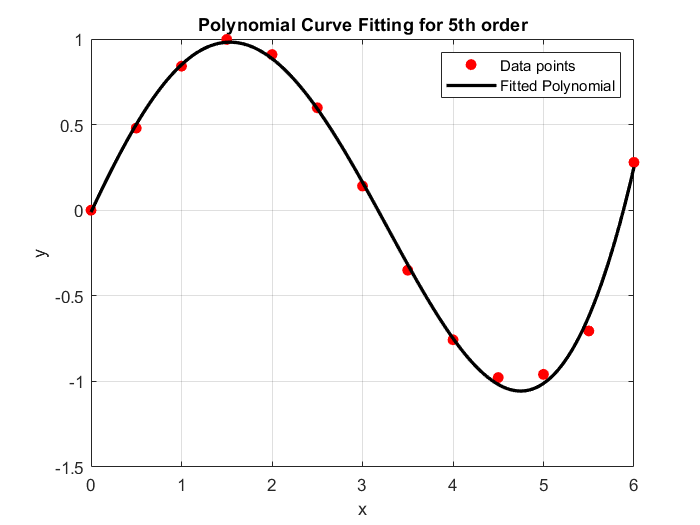
\includegraphics[width=1.1\linewidth]{Images/5}
		\caption{Curve fitting for $5^{th}$ order}
	\end{subfigure}
	
	\begin{subfigure}[t]{0.49\textwidth}
		\centering
		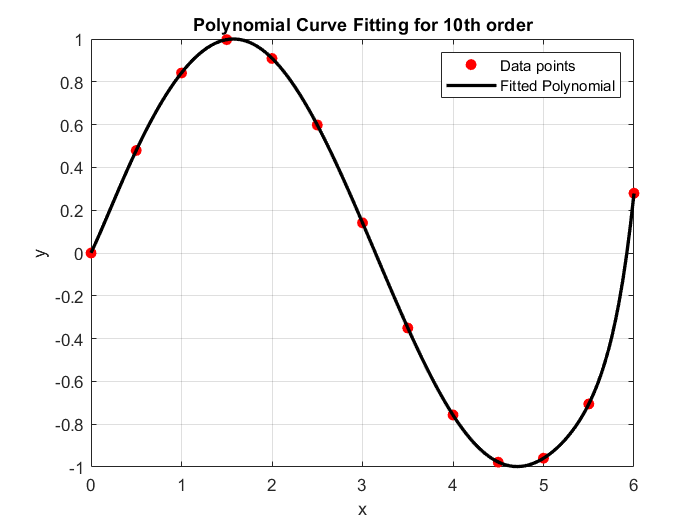
\includegraphics[width=1.1\linewidth]{Images/10}
	\caption{Curve fitting for $10^{th}$ order}
	\end{subfigure}
		\hfil
	\begin{subfigure}[t]{0.49\textwidth}
		\centering
		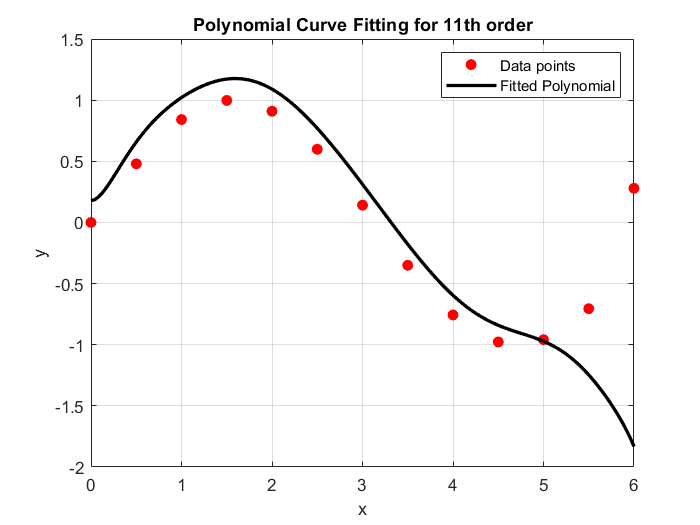
\includegraphics[width=1.1\linewidth]{Images/11}
		\caption{Curve fitting for $11^{th}$ order}
	\end{subfigure}
	\caption{Plot diagram for different order of polynomial curve fitting.}
\end{figure}
\newpage
	
	\section{Discussion}


	
	
	
		In this experiment, polynomial curve fitting was applied using various polynomial orders to approximate a set of data points. Polynomial curve fitting was applied using 2nd, 5th, 10th, and 11th order polynomials. The second-order fit resembled a straight line and failed to capture data variation, indicating under-fitting. The fifth-order polynomial provided a better fit by following the data more closely.
	
	The tenth-order polynomial gave the best result, accurately fitting the data with minimal deviation. However, the eleventh-order fit showed severe oscillations and poor accuracy due to \textbf{over-fitting}, where the curve attempted to pass through all points, causing instability. It was concluded that increasing the polynomial order improves fitting up to a point, after which over-fitting degrades performance.
	
	
\end{document}